\documentclass[12pt]{exam}         %% What type of document you're writing.

%%%%% Preamble

%% Packages to use

\usepackage{amsmath,amsfonts,amssymb}   %% AMS mathematics macros
\usepackage{lettrine}
\usepackage{graphicx}
\usepackage[export]{adjustbox}
\usepackage{tikz}
\usepackage{polyglossia}
\usepackage{xcolor}
\usepackage{longtable}
\usepackage{fontawesome}
\usepackage{hyperref}

\hypersetup{
    colorlinks=true,
    linkcolor=blue,
    filecolor=magenta,
    citecolor=blue,
    urlcolor=purple,
}

\setdefaultlanguage{english}
\setmainfont[Language=English]{Gentium Plus}

%% Title Information.

\title{The Term-end Fun Exam}
\author{Kedar Mhaswade, Free Learner's School}
\date{May 2021}

\setlength{\parindent}{0pt}% Remove paragraph indent
\usepackage[skip=\medskipamount]{parskip} % each paragraph has whitespace

\begin{document}

\maketitle

\lettrine[lines=3]{A}{LRIGHT}! The so-called term-end exam is here. Since we do everything for fun, we take exams lightly as well!  This text consists of problems that should be attempted for fun, but as part of an exam, so that you get used to the excitement, anxiety associated with it. After all, right now, exams is how the world tries to evaluate you. So, it helps you to get that experience. And you know, sometimes stress brings out our best response to it! 
The exam is based on what we have learned so far, however, that is just to be used as a guidance. Find out what \emph{kind} of problems are challenging and then perhaps work on the fundamentals to strengthen your understanding.


Some things to keep in mind:
\begin{enumerate}
\item It may be a good idea to print this out on both sides of a paper and attempt the answers with a pen or pencil on a separate paper. You may choose to use Google Docs instead as well. 
\item A quiz may contain errors. If a question is unclear, be sure to get it clarified.
\item It is a quiz of sorts. The time is not really limited, but you should plan on focusing for about an hour each time you take the quiz. Try to attempt the problems in a day, although make it a point to return to it from time to time. Remember, it is a marathon, not a 100-meter dash.
\item Give each problem enough thought and time and then present your solutions.
\item Have fun. Hopefully you will struggle to get through the problems. Perhaps you will make silly mistakes. Don't worry, it is all part of the game. You will get better only if you have fun doing it. Note that some problems may be difficult and you may be stuck. \emph{Being stuck is okay}. Note that some of these problems have been (or still are) difficult for me too.
\item For the sake of examination, the correct solution (however you find it) to every problem carries points indicated in a pair of parentheses. Giving points to solutions is, of course, pointless, but let's just do it for the sake of it and hope that we have some fun along the way. 
\item Be honest.
\end{enumerate}
\textbf{Good Luck}!

\newcommand\Prob[2]{%
   \leavevmode\par
   \stepcounter{question}
   \noindent
   Problem \thequestion \space (#2 points) -- #1 \par}

\newcommand\Ans[2][]{%
    \leavevmode\par\noindent
   {\leftskip37pt
    A --- \textbf{#1}#2\par}}

\newpage

\Prob{
See Figure \ref{fig: num-col}. Look at the way they are colored. 
\begin{figure}[h!]
    \centering
    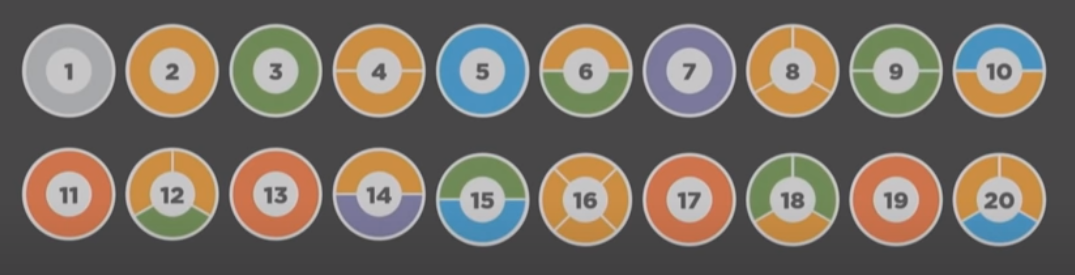
\includegraphics[width=0.5\linewidth]{numbers-and-colors.png}
    \caption{The First 20 Numbers}
    \label{fig: num-col}
\end{figure}

\begin{enumerate}
    \item How will you color numbers $21$, $22$, and $23$?
    \item Which is the first number after $1$ that will have a gray?
\end{enumerate}
}{2}

\Prob{
\begin{figure}[h!]
    \centering
    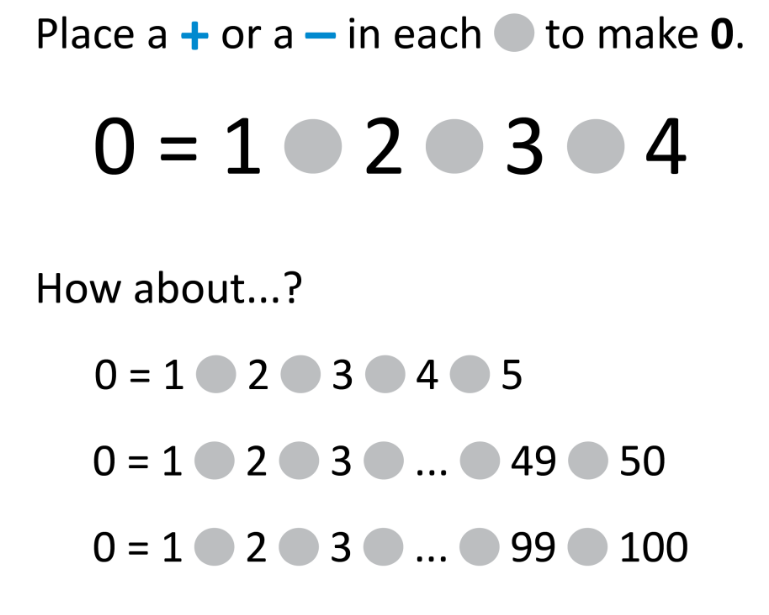
\includegraphics[width=0.5\linewidth, frame]{minus-plus.png}
    \caption{Minus Plus}
    \label{fig: minus-plus}
\end{figure}
    Solve the problem in Figure \ref{fig: minus-plus}. This is one of the things that mathematicians do: Generalization, wherein after solving a few concrete problems, they try to find a pattern. To achieve such a goal, they have to play with things at hand, just like what you are doing right now!
}{10}

\Prob{
    What is the difference between $(a^b)^{c}$ and $(a)^{b^c}$?
}{2}

\Prob{
    Find the values of $A$, $B$, and $C$ from the following sum:

    \begin{tabular}{cccc}
        & A & B & C \\
      + & A & B & C \\
      + & A & B & C \\
      \hline
        & B & B & B \\
    \end{tabular}
}{3}


\begin{thebibliography}{00}
    \bibitem{finkel} Dan Finkel. \href{https://www.ted.com/talks/dan_finkel_5_ways_to_share_math_with_kids/transcript?language=en}{TED Talk}.
    \bibitem{plus-minus} Glenn Stevens. \href{https://playwithyourmath.com/2020/02/09/24-plus-minus/}{Play With Your Math}.
\end{thebibliography}
\end{document}
